\begin{exercice*}[Parallélogramme]

    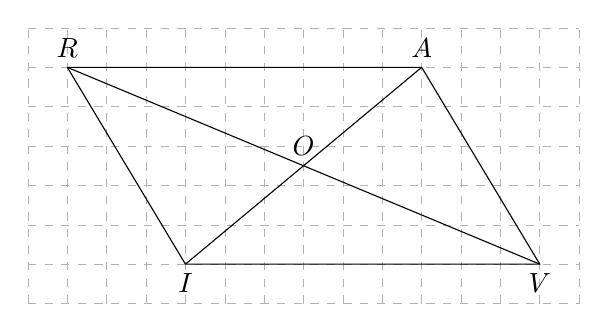
\begin{tikzpicture}[scale = 0.5]
        \draw[help lines, color=black!30, dashed] (0,0) grid (14,7);
        \coordinate[label=above:$R$] (R) at (1,6);
        \coordinate[label=above:$A$] (A) at (10,6);
        \coordinate[label=below:$V$] (V) at (13,1);
        \coordinate[label=below:$I$] (I) at (4,1);
        \coordinate[label=above:$O$] (O) at (7,3.5);
        \draw (R)--(A)--(V)--(I)--(R);
        \draw (R)--(V);
        \draw (I)--(A);
    \end{tikzpicture}

    % \begin{multicols}2
        \begin{enumerate}
            \item Coder les longueurs égales sur la figure.
            \item Déterminer les triangles égaux. Justifier.
        \end{enumerate}
    % \end{multicols}
\end{exercice*}
\begin{corrige}
    %\setcounter{partie}{0} % Pour s'assurer que le compteur de \partie est à zéro dans les corrigés
    % \begin{multicols}2
        \begin{enumerate}
            \item \phantom{rrr}
            
            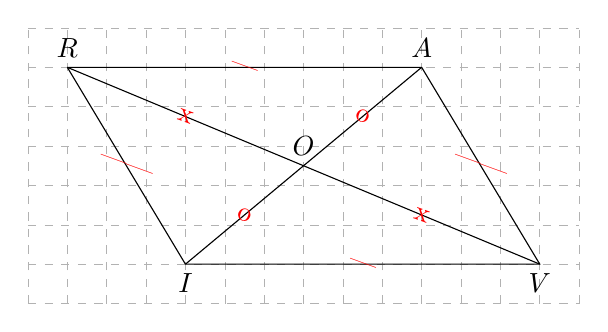
\begin{tikzpicture}[scale = 0.5]
                \draw[help lines, color=black!30, dashed] (0,0) grid (14,7);
                \coordinate[label=above:$R$] (R) at (1,6);
                \coordinate[label=above:$A$] (A) at (10,6);
                \coordinate[label=below:$V$] (V) at (13,1);
                \coordinate[label=below:$I$] (I) at (4,1);
                \coordinate[label=above:$O$] (O) at (7,3.5);
                \draw (R)--(A)--(V)--(I)--(R);
                \draw (R)--(V);
                \draw (I)--(A);
                \draw [color=red] (2.5,3.5) node[anchor = center, rotate = -20] {||};% (R)(I)
                \draw [color=red] (11.5,3.5) node[anchor = center, rotate = -20] {||};% (A)(V)
                \draw [color=red] (5.5,6) node[anchor = center, rotate = -20] {|};% (R)(A)
                \draw [color=red] (8.5,1) node[anchor = center, rotate = -20] {|};% (I)(V)
                \draw [color=red] (4,4.75) node[anchor = center, rotate = -20] {x};% (R)(O)
                \draw [color=red] (10,2.25) node[anchor = center, rotate = -20] {x};% (O)(V)
                \draw [color=red] (8.5,4.75) node[anchor = center, rotate = -20] {o};% (O)(A)
                \draw [color=red] (5.5,2.25) node[anchor = center, rotate = -20] {o};% (I)(O)
            \end{tikzpicture}            
            \item Dans un parallélogramme, les côtés opposés ont la même longueur et les diagonales ont le même milieu.
            
            D'où :            
            \begin{itemize}
                \item $RA=IV$, $OA=OI$ et $OR=OV$ donc \psshadowbox{$ROA$ et $OIV$ sont égaux}.
                \item $RI=AV$, $OI=OA$ et $OR=OV$ donc \psshadowbox{$ROI$ et $AOV$ sont égaux}.            
            \end{itemize}
        \end{enumerate}
    % \end{multicols}
\end{corrige}

